\documentclass[11pt,a4paper]{article}
\usepackage[latin1]{inputenc}
\usepackage[margin=1in]{geometry}
\usepackage{amsmath}
\usepackage{amsfonts}
\usepackage{amssymb}
\usepackage{graphicx}
\usepackage{enumitem}
\usepackage{listings}
\usepackage{color}

\definecolor{dkgreen}{rgb}{0,0.6,0}
\definecolor{gray}{rgb}{0.5,0.5,0.5}
\definecolor{mauve}{rgb}{0.58,0,0.82}

\lstset{frame=tb,
 language=MatLab,
 aboveskip=3mm,
 belowskip=3mm,
 showstringspaces=false,
 columns=flexible,
 basicstyle={\small\ttfamily},
 numbers=none,
 numberstyle=\tiny\color{gray},
 keywordstyle=\color{blue},
 commentstyle=\color{dkgreen},
 stringstyle=\color{mauve},
 breaklines=true,
 breakatwhitespace=true,
 tabsize=3
}

\setlength\abovedisplayskip{0pt}
\author{James Brissette}
\title{CS-6210: HW 4}
\begin{document}
	\maketitle
	
	\section{Chapter 6}
		\begin{itemize}
			\item[6.2]
				\begin{enumerate} [label={\alph*)}]
					\item Using the composite trapezoidal rule with four subintervals we find that $I_T$ can be calculated as follows:
					\begin{align*}
						I_T &= h\Big( \frac{1}{2}f_1 + f_2 + f_3 + f_4 + \frac{1}{2}f_5 \Big) \\
						    &= h\Big( \frac{1}{2}e^2 + e^1 + e^0 + e^{-1} + \frac{1}{2}e^{-2} \Big) \\
						    &\approx 3.9242
					\end{align*}
					In order to evaluate the error on this approximation, we need to find $\vert \vert f'' \vert \vert_\infty$:
					\begin{align*}
					\frac{d}{dx}\Big[e^{-2x}\Big]      &= -2e^{-2x} \\
					\frac{d^2}{dx^2}\Big[e^{-2x}\Big]  &= 4e^{-2x}
					\end{align*}
					\begin{align*}
					\vert \vert f'' \vert \vert_\infty &= max_{-1\leq x\leq 1} \vert 4e^{-2x} \vert\\
					\vert \vert f'' \vert \vert_\infty &= 4e^2
					\end{align*}
					Approximating our error we see:
					\begin{align*}
					\Biggl \vert \int_{-1}^{1}e^{-2x}dx - I_T \Biggl\vert &\leq \frac{2}{12}h^2 (4e^2) \\
					&\leq 1.2315
					\end{align*}
					
					\item We are able to use Simpson's rule in this case because the number of subintervals $n$ is even, and $I_S$ can be calculated as follows:
					\begin{align*}
						I_S &= \frac{h}{3}\Big(f_1 + 4f_2 + 2f_3 + 4f_4 + f_5 \Big) \\
							&= \frac{1}{6}\Big(e^2 + 4e^1 + 2 + 4e^-1 + e^-2 \Big) \\
							&\approx 3.6448
					\end{align*}
					In order to evaluate the error on this approximation, we need to find $\vert \vert f'''' \vert \vert_\infty$:
					\begin{align*}
					\frac{d^3}{dx^3}\Big[e^{-2x}\Big]  &= -8e^{-2x}  \\
					\frac{d^4}{dx^4}\Big[e^{-2x}\Big]  &= 16e^{-2x}
					\end{align*}
					\begin{align*}
					\vert \vert f'''' \vert \vert_\infty &= max_{-1eq x\leq 1} \vert 16e^{-2x} \vert\\
					\vert \vert f'''' \vert \vert_\infty &= 16e^2
					\end{align*}
					Approximating our error we see:
					\begin{align*}
					\Biggl \vert \int_{-1}^{1}e^{-2x}dx - I_S \Biggl\vert &\leq \frac{2}{90}h^4(16e^2) \\
					&\leq 0.1642
					\end{align*}
					
					\item Using the composite Hermite rule (or corrected trapezoidal rule) with four subintervals we find that $I_H$ can be calculated as follows:
					\begin{align*}
					I_H &= h\Big( \frac{1}{2}f_1 + f_2 + f_3 + f_4 + \frac{1}{2}f_5 \Big) + \frac{1}{12}h^2 (f'_1 - f'_{n+1}) \\
					&= \frac{1}{2}\Big( \frac{1}{2}e^2 + e^1 + e^0 + e^{-1} + \frac{1}{2}e^{-2} \Big) + \frac{1}{48}(-2e^{2} + 2e^{-2})\\
					&\approx 3.6219
					\end{align*}
					In order to evaluate the error on this approximation, we need to find $\vert \vert f'''' \vert \vert_\infty$ which was calculated previously:
					\begin{align*}
					\vert \vert f'''' \vert \vert_\infty &= 16e^2
					\end{align*}
					Approximating our error we see:
					\begin{align*}
					\Biggl \vert \int_{-1}^{1}e^{-2x}dx - I_H \Biggl\vert &\leq \frac{2}{720}h^4 (16e^2) \\
					&\leq 0.0205
					\end{align*}
					
					\item From Theorem 6.2, using the trapezoidal rule we use can substitute in the definition of our step $h$, $h=\frac{b-a}{n}$ in to the following equation for error:
					\begin{align*}
						\frac{2}{12}h^2 (4e^2) &\leq 10^{-6} \\
						h &\leq \Big( \frac{10^{-6}}{4e^2} \frac{12}{2} \Big)^{1/2} \\
						\frac{2}{n} &\leq \Big( \frac{10^{-6}}{4e^2} \frac{12}{2} \Big)^{1/2} \\
						n &\geq \frac{2}{\Big( \frac{10^{-6}}{4e^2} \frac{12}{2} \Big)^{1/2}}
					\end{align*}
					Solving this inequality yields $n \geq	4,439$
					
					\item From Theorem 6.3, using Simpson's rule we use can substitute in the definition of our step $h=\frac{b-a}{n}$ in to the following equation for error:
					\begin{align*}
					\frac{2}{90}h^4(16e^2) &\leq 10^{-6} \\
					h &\leq \Big( \frac{10^{-6}}{16e^2} \frac{90}{2} \Big)^{1/4} \\
					\frac{2}{n} &\leq \Big( \frac{10^{-6}}{16e^2} \frac{90}{2} \Big)^{1/4} \\
					n &\geq \frac{2}{\Big( \frac{10^{-6}}{16e^2} \frac{90}{2} \Big)^{1/4}}
					\end{align*}
					Solving this inequality yields $n \geq 81$
					
					\item From Theorem 6.4, using Simpson's rule we use can substitute in the definition of our step $h=\frac{b-a}{n}$ in to the following equation for error:
					\begin{align*}
					\frac{2}{720}h^4(16e^2) &\leq 10^{-6} \\
					h &\leq \Big( \frac{10^{-6}}{16e^2} \frac{720}{2} \Big)^{1/4} \\
					\frac{2}{n} &\leq \Big( \frac{10^{-6}}{16e^2} \frac{720}{2} \Big)^{1/4} \\
					n &\geq \frac{2}{\Big( \frac{10^{-6}}{16e^2} \frac{720}{2} \Big)^{1/4}}
					\end{align*}
					Solving this inequality yields $n \geq 48$
				\end{enumerate}
					
			\item[6.4]
				\begin{enumerate} [label={\alph*)}]
					\item Because we are given that $T=E\frac{du}{dx}$, we know that $\frac{du}{dx} = \frac{1}{E}T$. If we wanted to evaluate the the integral of  $\frac{du}{dx}$ in the interval $[0,1]$ we could write that as:
					\begin{align*}
						\int_{0}^{x}u'(x)\frac{d}{dx} &= \frac{1}{E}\int_{0}^{x}T(s)ds \\
						\frac{1}{E}\int_{0}^{x}T(s)ds &= u(x)\Big\vert_{0}^{x}
					\end{align*}
					or equivalently
					\begin{align*}
						u(x) - u(0) &= \frac{1}{E}\int_{0}^{x}T(s)ds \\
						u(x) &= u(0) + \frac{1}{E}\int_{0}^{x}T(s)ds
					\end{align*}
					
					\item To calculate $u(\frac{1}{4})$ using the trapezoidal rule and the data provided in table 6.10 we use the result from part a and set up the following:
					\begin{align*}
						u(1/4) = u(0) &+ \frac{1}{E} \int_{0}^{\frac{1}{4}} T(s)ds \quad where \quad u(0)=0,E=4\\
						u(1/4) &= 0 + \frac{1}{4}* \frac{1}{4}\Big(\frac{1}{2}(1)+\frac{1}{2}(-1)\Big) \\
						u(1/4) &= 0
					\end{align*}
					We use the trapezoidal rule similarly to calculate $u(1/2)$, $u(3/4),$ and $u(1)$ using the same values of $u(0)$ and $E$:
					\begin{align*}
						u(1/2) &= 0 + \frac{1}{4} \int_{0}^{\frac{1}{2}} T(s)ds\\
						u(1/2) &= 0 + \frac{1}{4}* \frac{1}{4}\Big(\frac{1}{2}(1)+(-1)+\frac{1}{2}(2)\Big) \\
						u(1/2) &= \frac{1}{32}\\
						\\
						u(3/4) &= 0 + \frac{1}{4} \int_{0}^{\frac{3}{4}} T(s)ds\\
						u(3/4) &= 0 + \frac{1}{4}* \frac{1}{4}\Big(\frac{1}{2}(1)+(-1)+(2)+\frac{1}{2}(3)\Big) \\
						u(3/4) &= \frac{3}{16}\\
						\\
						u(1) &= 0 + \frac{1}{4} \int_{0}^{1} T(s)ds\\
						u(1) &= 0 + \frac{1}{4}* \frac{1}{4}\Big(\frac{1}{2}(1)+(-1)+(2)+(3)+\frac{1}{2}(4)\Big) \\
						u(1) &= \frac{13}{32}
					\end{align*}
					\item In order to use the composite midpoint rule to evaluate $u(1)$ we need the values of the midpoints of each step. Since we're not give the value of the function at $x=\frac{1}{8}$, we must increase our step size from $\frac{1}{4}$ to $\frac{1}{2}$ so we are able to use the data that is provided as our midpoints: 
					\begin{align*}
						u(1) &= 0 + \frac{1}{4} \int_{0}^{1} T(s)ds\\
						u(1) &= 0 + \frac{1}{4} I_M \\
						u(1) &= 0 + \frac{1}{4}* \frac{1}{2}\Big((-1)+(3)\Big)\\
						u(1) &= \frac{1}{4}
					\end{align*}
					\item We can use Simpson's rule to evaluate $u(1)$ since the number of intervals $n$ is even:
					\begin{align*}
					u(1) &= 0 + \frac{1}{4} \int_{0}^{1} T(s)ds\\
					u(1) &= 0 + \frac{1}{4} I_S \\
					u(1) &= 0 + \frac{1}{4}* \frac{1}{12}\Big((1)+4(-1)+2(2)+4(3)+(4)\Big)\\
					u(1) &= \frac{17}{48}
					\end{align*}
					\item If we use our result from part b we see $I_T = \frac{13}{8}$ and we use this in place of $I_T(2n)$. Following the theorem in the book we find that the Romberg Integration using the trapezoidal rule takes the form:
					$$\int_{a}^{b} f(x)dx = \frac{4}{3}I_T(2n)-\frac{1}{3}I_T(n)+O(h^3)$$
					Solving for $I_T(n)$ we get: 
					\begin{align*}
						I_T(n) &= \frac{1}{2}\Big(\frac{1}{2}(1) + (2) + \frac{1}{2}(4)\Big)\\
						I_T(n) &= \frac{9}{4}
					\end{align*}
					Putting it all together we see:
					\begin{align*}
						u(1) &= \frac{4}{3}(\frac{13}{8})-\frac{1}{3}(\frac{9}{4})\\
						u(1) &= \frac{17}{12}
					\end{align*}
					
				\end{enumerate}
				
			\item[6.8]
				\begin{enumerate} [label={\alph*)}]
					\item Using the trapezoidal rule, we know our error terms looks like the following (evaluated at $erf(2)$):
					\begin{align*}
						\Biggl \vert \frac{2}{\sqrt{\pi}} \int_{0}^{2}e^{-s^2}ds \Biggl\vert &\leq \frac{2}{12}h^2 \vert \vert (4x^2-2)e^{-x^2} \vert \vert_\infty
					\end{align*}
					Taking the norm of $\vert \vert f'' \vert \vert_\infty$ to be $.8925$ (solved using MATLAB), we solve for $h$:
					\begin{align*}
						\frac{2}{12}h^2 (.8925) &\leq 10^{-6}\\
						h &\leq \sqrt{\frac{10^{-6}}{.8925}*6} \\
						h &\leq  2.592815e-03
					\end{align*}
					\item Issue with this MATLAB code. Not particularly close to the true value..
							\begin{lstlisting}
						function [output] = ch6q8()
						% Solves for h using the trapezoidal rule
						x = 2;
						IT = 0;
						
						erf2 = 0.995322265;
						
						error = 1;
						n = 200000;
						while abs(error) > 10e-7
						% while n < 10
						h = x/n;
						%     fprintf('N = %d; Step size is %d; ',n, h);
						IT = (.5*exp(0) + .5*(1/exp((2)^2)));
						%     fprintf('Intermediate eval at ');
						for i = 1:n-1
						IT = IT + (1/ exp((i*h)^2));
						%         fprintf('x = %d; ',(i)*h);
						end
						IT = IT * h;
						error = erf2 - IT
						n = n+1;
						end
						end
						\end{lstlisting}
					\item Using Simpson's rule, we know our error terms looks like the following (evaluated at $erf(2)$):
					\begin{align*}
					\Biggl \vert \frac{2}{\sqrt{\pi}} \int_{0}^{2}e^{-s^2}ds \Biggl\vert &\leq \frac{2}{90}h^4 \vert \vert f'''' \vert \vert_\infty
					\end{align*}
					In this case, finding $f''''$ is not as trivial, so we include the process:
					\begin{align*}
						\frac{d^2}{dx^2}f(x) &= (4x^2-2)e^{-x^2} \\
						\frac{d^3}{dx^3}f(x) &= -2x(4x^2-2)e^{-x^2} + 8xe^{-x^2} \\
						 &= (-8x^3+12x)e^{-x^2} \\
						\frac{d^4}{dx^4}f(x) &= (-24x^2+12)e^{-x^2} + -2x(-8x^3+12x)e^{-x^2} \\
						&= (-16x^4 - 48x^2 +12)e^{-x^2} 
					\end{align*}
					If we plot each these curves we can see at $f''''$ the maximum value is obtained when $x=0$ and $\vert \vert f'''' \vert \vert_\infty = 12$:
					\begin{center}
						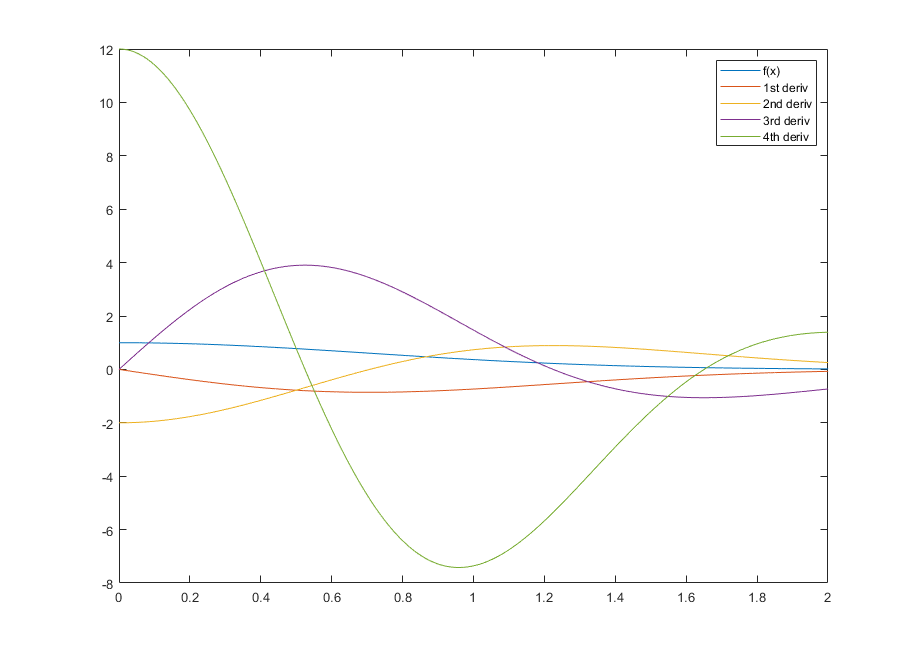
\includegraphics[width=1\linewidth]{ch6q8c}
					\end{center}
					Taking the norm of $\vert \vert f'''' \vert \vert_\infty$ to be $12$ (solved using MATLAB), we solve for $h$:
					\begin{align*}
					\frac{2}{90}h^4 (12) &\leq 10^{-6} \\
					h &\leq \sqrt[4]{\frac{10^{-6}}{12}*\frac{90}{2}} \\
					h &\leq 4.4005587e-02
					\end{align*}
					\item Using the same code from part B adapted for Simpson's rule...
				\end{enumerate}
				
			\item[6.15]
				\begin{enumerate} [label={\alph*)}]
					\item 
					\item 
					\item 
					\item
				\end{enumerate}
			
			\item[6.18]
				\begin{enumerate} [label={\alph*)}]
					\item 
					\item
				\end{enumerate}
				
			\item[6.19]
				\begin{enumerate} [label={\alph*)}]
					\item 
					\item 
					\item
				\end{enumerate}
				
			\item[6.20]
				\begin{enumerate} [label={\alph*)}]
					\item 
					\item 
					\item
				\end{enumerate}
				
			\item[6.21]
				\begin{enumerate} [label={\alph*)}]
					\item 
					\item
				\end{enumerate}
		\end{itemize}	
	
\end{document}